\section{Webcam-Steuerung}
Zur Wetterstation Arbon gehört eine schwenk- und zoombare Webcam. Diese ist über ein Applikations-Plugin in die Webseite integriert. In der Titelleiste sind die wichtigsten Wetterdaten aufgeführt, wobei die Einheit der Windgeschwindigkeit jeweils alle dreissig Sekunden zwischen km/h und Knoten wechselt. Die Webseite der Webcam ist in Abbildung \ref{img:warteschlange} links dargestellt.

\begin{figure}[h]
	\centering
	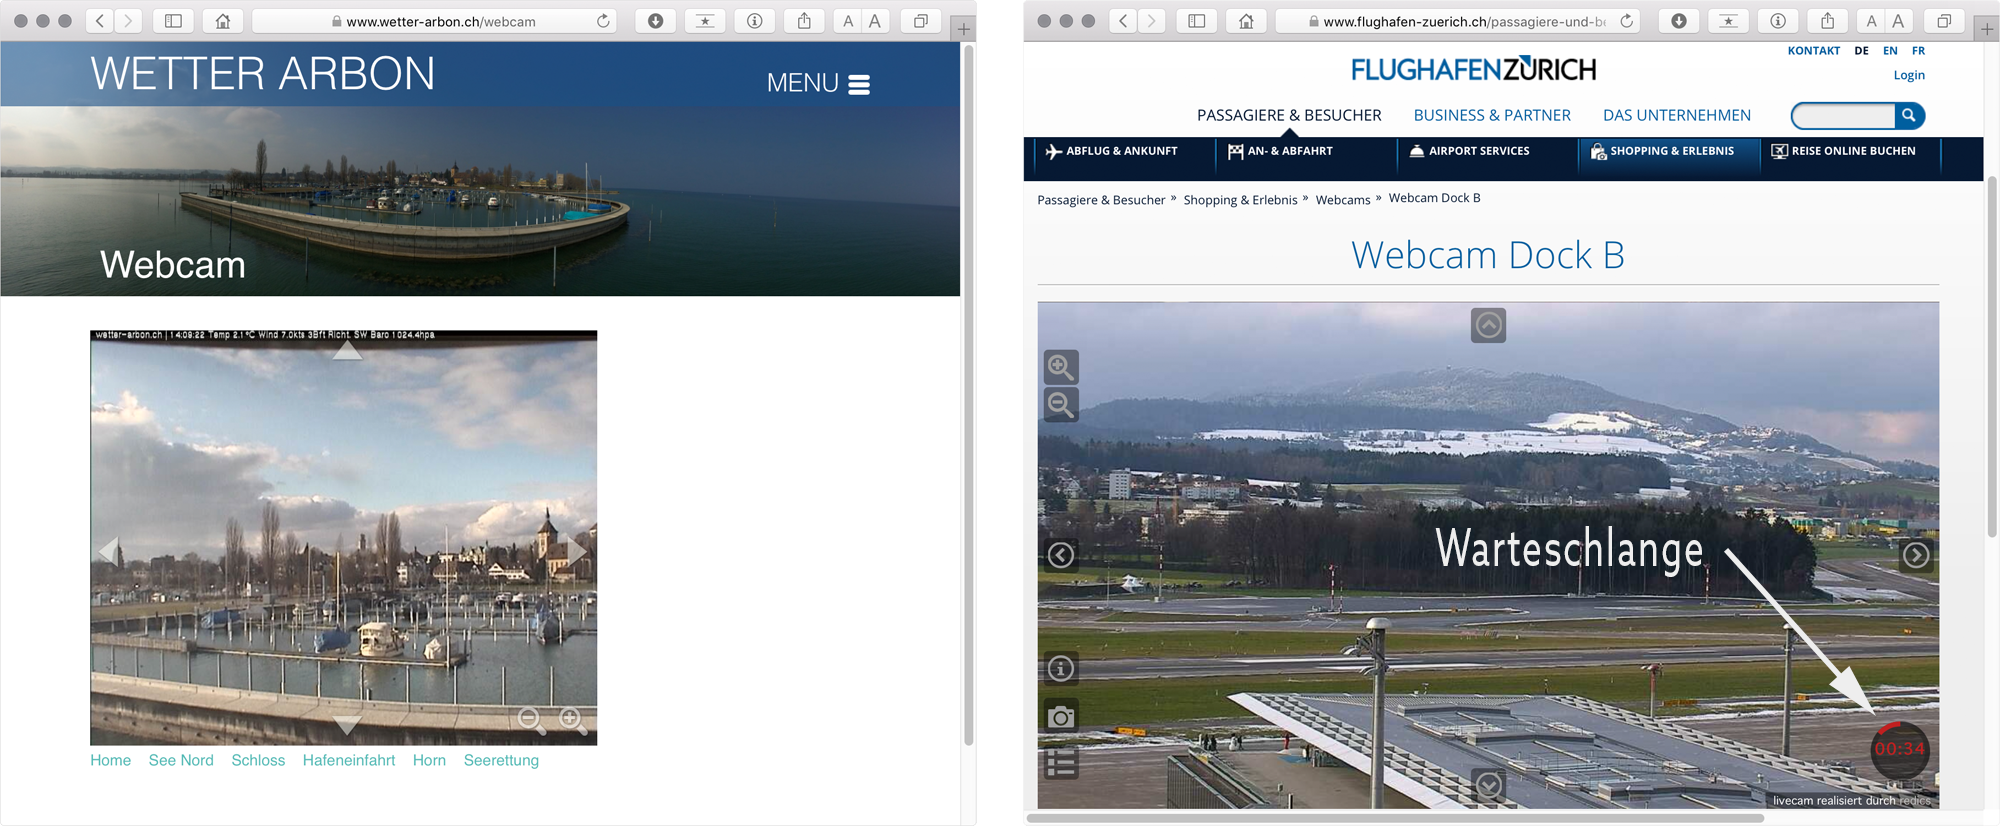
\includegraphics[width=1\linewidth]{img/warteschlange}
	\caption{Webcam Arbon und Beispiel einer Warteschlange}
	\label{img:warteschlange}
\end{figure}


% Positionierung / Abfrage der Position
Der Benutzer hat die Möglichkeit die Webcam nach oben/unten und nach links/rechts zu bewegen. Sechs voreingestellte Positionen stehen als Shortlinks zur Verfügung. Diese Positionen sind in der Betriebseigenen Software konfiguriert. Die freie Positionierung erfolgt über Pfeile, sowie die Plus und Minus am Bildrand, je nachdem welcher Button geklickt wird, sendet die Webseite das Kommando mittels HTTP an die Webcam. Die Zusammenstellung der URL geschieht über ein Javascript, wie man dem Code in Listing \ref{lst:cam} entnehmen kann.

\begin{lstlisting}[caption={Positionsänderung der Webcam},label={lst:cam},language=html]
 <div class="container webcam" id="webcam_585">
	<img class="pageImage" src="https://webcam.wetter-arbon.ch/mjpg/video.mjpg"/>
</div>
<script type="text/javascript">
	function changeWebCam(command) {
		var urlAddition;
		switch (command) {
			case 'up':
			case 'down':
			case 'left':
			case 'right':
			case 'home':
				urlAddition = 'move=' + command;
				break;
				
			case 'zoomIn':
				urlAddition = 'rzoom=2500';
				break;
				
			case 'zoomOut':
				urlAddition = 'rzoom=-2500';
				break;
				
			case 'Hafeneinfahrt':
				urlAddition = 'gotoserverpresetname=' + command;
				break;		
		}
		console.log('changeWebCam');
		$.get('https://webcam.wetter-arbon.ch/axis-cgi/com/ptz.cgi?camera=1&' + urlAddition);
	}
\end{lstlisting}


% Zoom
\subsection{Positionsabhängige Zoombeschränkung}
In der betriebseigenen Software lassen sich viele Parameter konfigurieren, unter anderem der Zoomfaktor. Das Problem ist hier, dass der Zoomfaktor in der betriebseigenen Software nur allgemein eingestellt werden kann, das heisst die Beschränkung gilt immer, egal ob die Kamera auf eine Wohnung zeigt oder auf den See raus. Aus Perönlichkeitsschutz-Gründen musste deshalb der Zoomfaktor auf die 4-fache Vergrösserung limitiert werden, möglich wäre aber eine 216-fache Vergrösserung. Daraus wird deutlich, dass die Webcam eigentlich viel mehr Potential hat. Die Idee ist nun die Limitierung des Zooms so zu konfiguriert, dass diese möglichst dynamisch ist. Das heisst, dass je nach Position die Zoom-Limitierung ändert. Der Zoom soll, vor allem auf den See hinaus, in vollem Umfang genutzt werden können. Die Ausrichtung der Kamera kann mit einer einfachen HTTP GET Anfrage abgerufen werden. So kann mittels Javascript der Zoom beschränkt oder erweitert werden

% Warteschlange
\subsection{Warteschlange für Webcam-Steuerung}
Die Möglichkeit der Webcam-Steuerung übers Web ist zwar sehr attraktiv, hat aber auch seine Nachteile. Zum Beispiel wenn mehrere Personen gleichzeitig auf die Webcam zugreifen. Zur Zeit ist es so dass, die HTTP-Request der Reihe nach abgearbeitet werden. Es ist also möglich, dass sich die Benutzer gegenseitig in der Bedienung stören, was unter Umständen recht mühsam ist. Das Prinzip der Warteschlange kann hier Abhilfe schaffen. Jeder Benutzer erhält eine besitmmte Zeit den alleinigen Zugriff auf die Steuerung der Webcam. So eine Lösung setzt zum Beispiel der Flughaben Zürich ein, wie in Abbildung \ref{img:warteschlange} rechts dargestellt.


